\documentclass[12pt]{extarticle}
\usepackage[utf8]{inputenc}
\usepackage{graphicx}
\usepackage{float}
\usepackage{array}
\usepackage{makecell} %line breaks inside table cells
\usepackage{changepage} %temp adjust margins
\usepackage[table]{xcolor} %color tables
\usepackage{outlines}
\usepackage{multirow}
\usepackage{caption}
\usepackage{etoolbox}
\usepackage[margin=1in]{geometry}
\usepackage{tabularx}
\usepackage{titling}
\usepackage{titlesec}
\usepackage{helvet}
\usepackage{indentfirst}
\usepackage{arydshln} %dashed lines (must load in last)

\BeforeBeginEnvironment{tabular}{\fontsize{10}{12}\selectfont}
\AfterEndEnvironment{tabular}{}
\BeforeBeginEnvironment{tabularx}{\fontsize{10}{12}\selectfont}
\AfterEndEnvironment{tabularx}{}


\graphicspath{ {img/} }

\titleformat*{\section}{\bfseries\sffamily\fontsize{14}{16}\selectfont}
\titleformat*{\subsection}{\bfseries\sffamily\fontsize{12}{14}\selectfont}
\titleformat*{\subsubsection}{\bfseries\sffamily\fontsize{12}{14}\selectfont}

%\captionsetup[table]{font={sf, normalsize}}

\renewcommand{\baselinestretch}{1.1} 



\begin{document}



\definecolor{highlight}{HTML}{9DE6AA} %grudsbo green, light edition
\definecolor{maroon}{cmyk}{0,0.87,0.68,0.32}
\definecolor{badhighlight}{HTML}{FF0000}


\title{GroundsBot: Autonomous Golf Course Maintenance \\[.5ex]
		\Large Conceptual Design Review}
\date{September 2017}
\author{CMU MRSD Team A        \\ Sponsor: Discovery Robotics \\ David Evans \\
        Adam Driscoll \\ Henry Chen  \\
        Josh Bennett  \\ Joe Phaneuf \\ }

\maketitle
\def\svgwidth{\columnwidth}
\input{img/groundsbot_logo.pdf_tex}
\newpage

\tableofcontents
\newpage

\newpage
\section{Project Description}

People spend a lot of time mowing grass. This is particularly true for golf courses. Golf courses have hundreds of acres of land requiring careful maintenance.  The median club in the United States spends \$1.2 million per year on maintenance \cite{clubbenchmarking}. A Pittsburgh area golf course superintendent \cite{interview-duxbury} revealed that his staff spends 65\% of their time mowing, and 60\% of that time is spent just on the rough. This is an industry ripe for automation.
\\

Autonomous mowers are commercially available today, however most of these units require buried wires, beacons, or extensive mapping to provide boundaries. For a golf course, the mowing area is so large that those setup methods are a barrier to deployment. The GroundsBot team aims to deliver an autonomous mower that can be deployed with minimal infrastructure, using a coarse boundary map provided by the user.

\newpage
\section{Use Case}
\begin{table}[H]
  \def\arraystretch{5}


\begin{tabular}{cl}
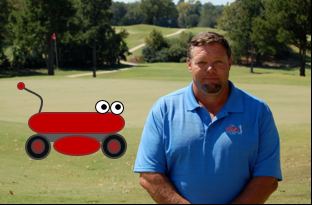
\includegraphics[width=6cm]{usecase1_1.png} \\
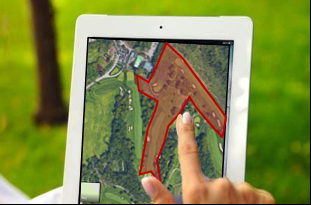
\includegraphics[width=6cm]{usecase1_2.png} \\
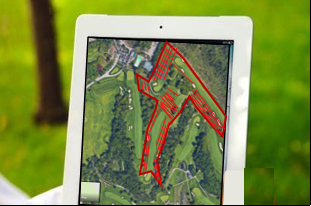
\includegraphics[width=6cm]{usecase1_3.png} \\
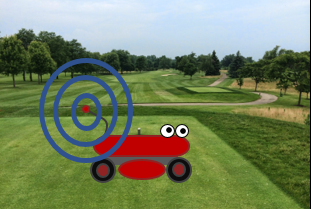
\includegraphics[width=6cm]{usecase1_4.png} \\
\end{tabular}
\end{table}

\begin{table}[H]
  \def\arraystretch{5}

\begin{tabular}{cl}
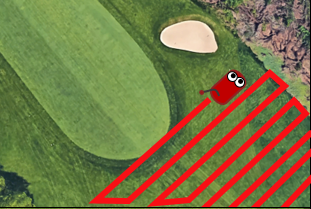
\includegraphics[width=6cm]{usecase1_5.png} \\
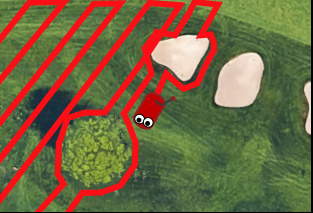
\includegraphics[width=6cm]{usecase1_6.png} \\
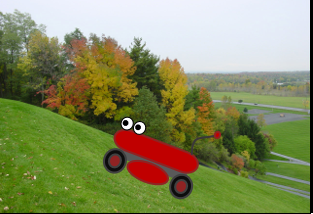
\includegraphics[width=6cm]{usecase1_7.png} \\
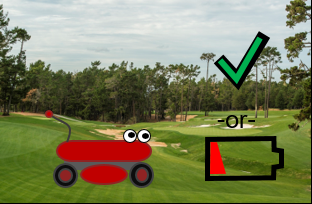
\includegraphics[width=6cm]{usecase2_1.png} \\

\end{tabular}
\end{table}

\begin{table}[H]
  \def\arraystretch{5}

\begin{tabular}{cl}
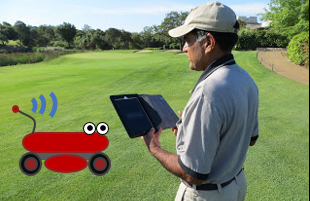
\includegraphics[width=6cm]{usecase2_2.png} \\
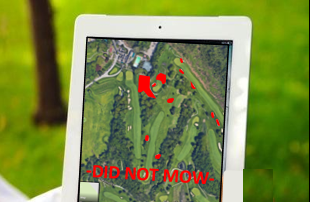
\includegraphics[width=6cm]{usecase2_3.png} \\
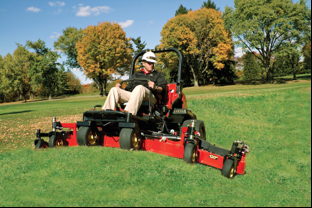
\includegraphics[width=6cm]{usecase2_4.png} \\
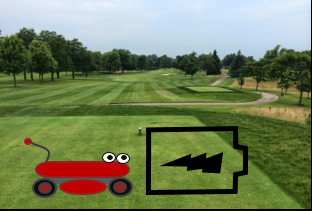
\includegraphics[width=6cm]{usecase2_5.png} \\

\end{tabular}
\end{table}

\newpage
\section{System Level Requirements}

The system requirements were decided upon to demonstrate a proof of concept autonomous lawn mower that can be set up with minimal added infrastructure. The only added infrastructure will be a docking station for GroundsBot. To accomplish this, GroundsBot must be able to localize with extreme accuracy in an unknown environment. GroundsBot must also be able to navigate consistently along a mowing path plan. Finally, GroundsBot must be able to detect and avoid any obstacles along the way.

\subsection{Mandatory Requirements}
\begin{center}
  \begin{table}[H]
  \caption{Mandatory Performance Requirements}
  \label{table:mandatory performance}
  
  \vspace{1em}

  \def\arraystretch{1.5}
  	\begin{tabularx}{\textwidth}{ lXX }
  	  	\hline
		\textbf{ID} & \textbf{Requirement} & \textbf{Description} \\
    	M.P.1 &
    	First time user inputs map within 15 minutes &
    	GroundsBot should be easy to use \\
   		M.P.2 &
   		System returns proposed route/coverage map within 5 minutes &
   		Related to M.P.1, GroundsBot should start up quickly to ease the mind of the user \\
   		M.P.3 &
   		Cut 0-25\% overlap for 95\% of grass &
   		When mowing, GroundsBot should cut in a way that accomplishes full grass coverage while maintaining efficiency by reducing overlap\\
		M.P.4 &
		Mow 50$ft^2$ of 30 degree sloped grass &
		GroundsBot should be able to handle steep slopes to eliminate safety hazards \\
		M.P.5 &
		Detect 80\% of objects greater than 27 cubic inches &
		GroundsBot should be able to recognize obstacles in order to prevent collisions and mowing accidents \\
		M.P.6 &
		Mow to within 1 foot of detected obstacles &
		GroundsBot should be able to detect an obstacle (M.P.5) and navigate around it to continue its mowing path \\
		M.P.7 &
		Mow 90\% of a $\frac{1}{4}$ acre area &
		GroundsBot will encounter obstacles along the way preventing it from 100\% coverage \\
	\end{tabularx}
  \end{table}
\end{center}

\subsection{Desirable Performance Requirements}
\begin{center}
  \begin{table}[H]
  \caption{Desirable Performance Requirements}
  \label{table: desirable performance}
  
  \vspace{1em}

  \def\arraystretch{1.5}
  \begin{tabularx}{\textwidth}{ lXX }
      \hline
	  \textbf{ID} & \textbf{Requirement} & \textbf{Description} \\
	  D.P.1 &
	  Mow to within 3 inches of a detected obstacles &
	  A stretch goal for when M.P.6 (mow within 1 ft. of obstacles) is achieved \\
  	  D.P.2 &
  	  Visually report mowing coverage and obstacles encountered &
  	  GroundsBot should report areas it missed to the user so the user knows where to manually mow to achieve full coverage\\
  \end{tabularx}
  \end{table}
\end{center}

\subsection{Mandatory Non-Functional Requirements}
\begin{center}
  \begin{table}[H]
   \caption{Mandatory Non-Functional Requirements}
    \label{table: mandatory non-functional}
    
    \vspace{1em}

    \def\arraystretch{1.5}
    \begin{tabularx}{\textwidth}{ lXX }
     \hline
  	 \textbf{ID} & \textbf{Requirement} & \textbf{Description} \\
	  M.N.1 &
  	  Return home to within 5 feet of dock &
  	  GroundsBot should return to its starting position to remove as much hassle from the user as possible \\  	  
  	  M.N.2 &
  	  Have a functional and easily accessible emergency stop &
  	  GroundsBot should be safe to use and easy to shut down in case of emergency\\
  	  M.N.3 &
  	  Be clearly visible &
  	  GroundsBot should indicate its presence and status to everyone nearby \\
  	  M.N.4 &
  	  Do not tear up grass &
  	  GroundsBot should not ruin any area it travels over \\
  	\end{tabularx}
  \end{table}
\end{center}

\subsection{Desirable Non-Functional Requirements}
\begin{center}
  \begin{table}[H]
  	\caption{Desirable Non-Functional Requirements}
  	\label{table: desirable non-functional}
  	\vspace{1em}

  	\def\arraystretch{1.5}
	\begin{tabularx}{\textwidth}{ lXX }
  	\hline
  	  \textbf{ID} & \textbf{Requirement} &
  	  \textbf{Description} \\
  	  D.N.1 &
  	  Operates in variable lighting conditions &
  	  GroundsBot should operate at night to avoid interrupting golfers\\
  	  D.N.2 &
  	  Deck adjustable 0.5” to 2” &
  	  GroundsBot should be able to meet the grass height standards of different golf courses\\
  	  D.N.3 &
  	  Bot is resistant to impacts &
  	  GroundsBot should be unaffected if hit by a golf ball while mowing\\
  	  D.N.4 &
  	  Return home to and mate with charging dock &
  	  A stretch goal if M.N.1 (return to within 5 ft. of dock) is achieved \\
	\end{tabularx}
  \end{table}
\end{center}


\newpage
\section{Functional Architecture}
  There are three sub-systems that combine to accomplish the functionality needed for GroundsBot (Figure~\ref{fig:functional}). The User Interface accepts inputs from the groundskeeper, generating detailed mowing regions. The Charging Dock acts as a home point for charging the robot, while also providing a reference signal for correcting localization issues. The Mowing Robot includes internal sub-systems which enable the robot to navigate the golf course, cut the rough, and return to the charging dock when needed.\\
  
\begin{figure}[H]
\centering
\def\svgwidth{\columnwidth}
\input{img/functional.pdf_tex}
\caption{Functional Architecture}
\label{fig:functional}
\end{figure}

  The Mowing Robot sub-system is responsible for many critical tasks in the Autonomous Golf Rough Mowing system The Mowing Platform is one internal sub-system that ensures effective mowing operations by storing energy, providing mobility, and docking when charging is needed. The Platform Electronics sub-system provides electrical controls for the motors and hosts the computing resources needed to run the algorithms for mowing. The sensor data provided by this sub-system is crucial for the remaining systems, enabling full mowing autonomy.\\
  
  The remaining sub-systems within the Mowing Robot include Online Perception, Robot Localization, Navigation Planning, and Control. These software systems provide GroundsBot with awareness of surroundings, knowledge of position, and in-depth details about the grass. This enables successful navigation through complicated environments, and provides the information necessary to control GroundsBot effectively.\\

\newpage
\section{System Level Trade Studies}
	\subsection{Platform Trade Study}


     \begin{table}[H]
		
		
		\caption{Platform Configuration Diagrams}
		\label{PlatformConfigDiagramsTable}
		\begin{adjustwidth}{-1in}{-1in}
		\centering
		\setlength{\dashlinedash}{.5pt}
		\setlength\tabcolsep{4pt}
		\def\arraystretch{1.9}
		

		\begin{tabular}{lcccccccc}
		\hline
        \makecell{\textbf{Configuration}\\ \textbf{Name}} & \makecell{\\ \textbf{Description}} & \makecell{\\ \textbf{Diagram}}  \\ 
		\makecell[l]{4 Wheel \\ Skid} &  \makecell[l]{Four driven wheels \\ with skid steering.} &  \makecell[l]{\\ 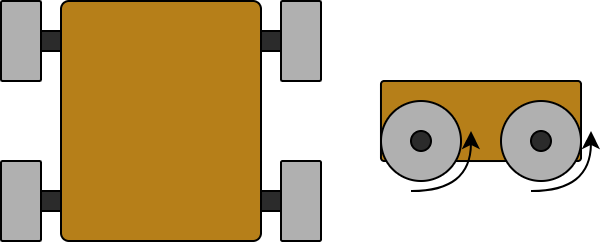
\includegraphics[width=4cm]{4_wheel_skid}} \\  
		\makecell[l]{2 Wheel \\ Differential \\ with Casters} &  \makecell[l]{Two driven wheels \\ with casters for free \\ rotation.} &  \makecell[l]{\\ 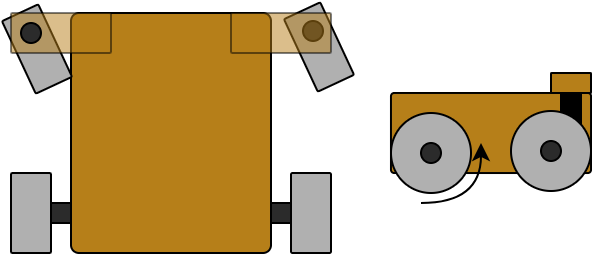
\includegraphics[width=4cm]{2_wheel_diff}} \\
		\makecell[l]{AWD \\ Standard \\ Steering} &  \makecell[l]{Four driven wheels \\ with standard \\differential steering.} &  \makecell[l]{\\ 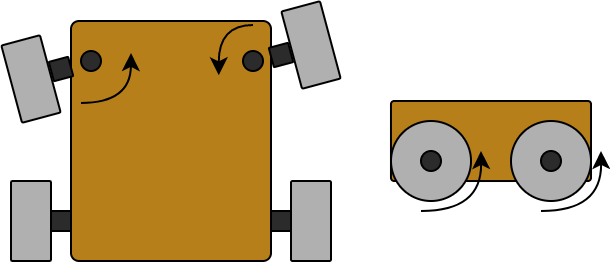
\includegraphics[width=4cm]{awd_standard_steer}} \\
		\makecell[l]{RWD \\ Standard \\ Steering} &  \makecell[l]{Two driven wheels \\ with standard\\ differential steering.} &  \makecell[l]{\\ 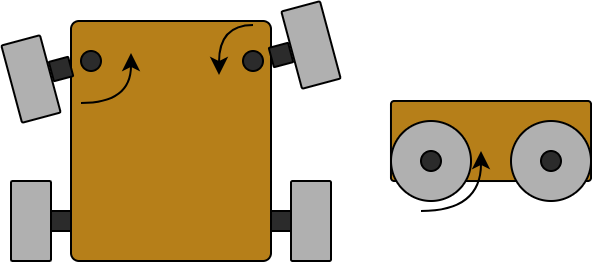
\includegraphics[width=4cm]{rwd_standard_steer}} \\
		\makecell[l]{Articulated} &  \makecell[l]{Four driven wheels \\ with center pivot \\ articulated steering.} &  \makecell[l]{\\ 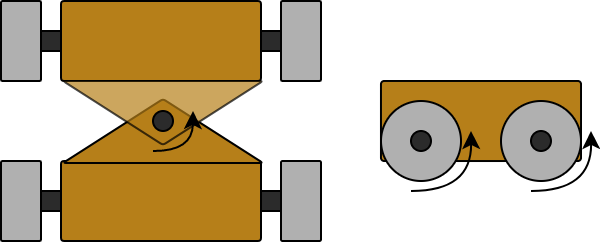
\includegraphics[width=4cm]{articulated}} \\
		\makecell[l]{Tracked} &  \makecell[l]{Two driven wheels \\ with tracks and \\ skid steering.} &  \makecell[l]{\\ 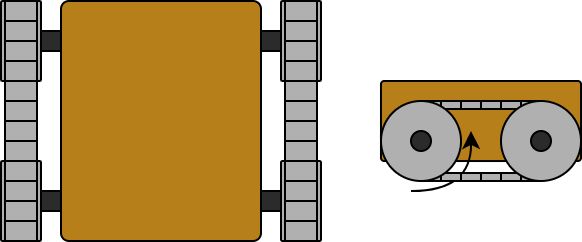
\includegraphics[width=4cm]{tracked}} \\
		\makecell[l]{3 Wheel \\ Delta} &  \makecell[l]{Three driven wheels \\ with immediate x, y, \\ and rotation control.} &  \makecell[l]{ 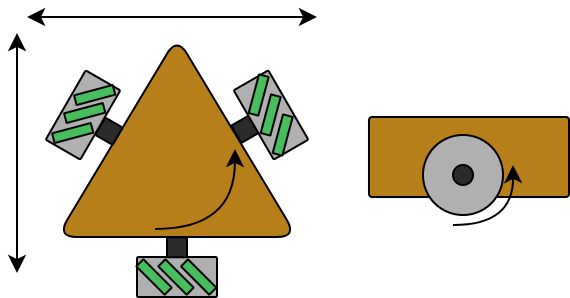
\includegraphics[width=4.1cm]{3_wheel_delta}} \\
		\makecell[l]{4 Wheel \\ Omniwheel} &  \makecell[l]{Four driven wheels \\ with immediate x, y, \\ and rotation control.} &  \makecell[l]{\\ 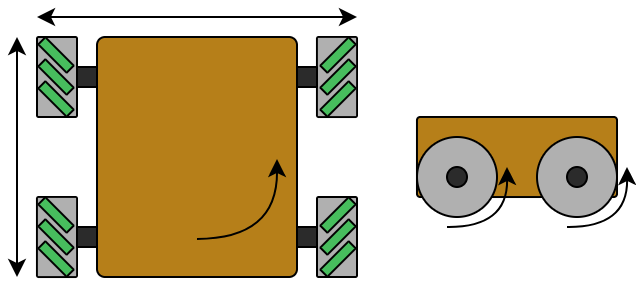
\includegraphics[width=4.3cm]{4_wheel_omniwheel}} \\
		
        \end{tabular}
		
		\end{adjustwidth}
		\end{table}





%%%%%%%%%%%%%%platform config table%%%%%%%%%%%%%%%%%%%%%%%%	
		\begin{table}[H]
		
		
		\caption{Platform Configuration Trade Study}
		\label{PlatformConfigTable}
		\begin{adjustwidth}{-1in}{-1in}
		\centering
		\setlength{\dashlinedash}{.5pt}
		\setlength\tabcolsep{4pt}
		\def\arraystretch{1.9}
		
		\vspace{1em}

		\begin{tabular}{lcccccccc}
		\hline
		                                                                                  & \makecell{\\ \\ \textbf{Speed}} & \makecell{\\ \textbf{Wheel} \\ \textbf{Compaction}} & \makecell{\\ \\ \textbf{Stability}} & \makecell{\\ \textbf{Platform} \\ \textbf{Complexity}} & \makecell{\\ \textbf{Odometry} \\ \textbf{Accuracy}} & \makecell{\\ \textbf{Turning} \\ \textbf{Radius} } & \makecell{\textbf{Performance} \\ \textbf{on Uneven} \\ \textbf{Terrain}} & \makecell{\\ \\ \textbf{Score}} \\ 
		\makecell[l]{Weights \\ (1-5)}                                            & 3     & 2                & 1         & 3                   & 4                 & 5                                          & 5                             &       \\ \hline
		
		\\[-3ex]
		\makecell[l]{4 Wheel \\ Skid}                                             & 5     & 4                & 4         & 4                   & 1                 & 1                                          & 5                             & 73    \\ \hdashline 
		
		%jesus christ this row is a goddamn mess BUT YOU GOTTA DO WHAT YOU GOTTA DO
		\cellcolor{highlight}\makecell[l]{2 Wheel \\ Differential \\ with Casters}& \multicolumn{1}{c}{\cellcolor{highlight}4} & \multicolumn{1}{c}{\cellcolor{highlight}3} & \multicolumn{1}{c}{\cellcolor{highlight}4} & \multicolumn{1}{c}{\cellcolor{highlight}5} & \multicolumn{1}{c}{\cellcolor{highlight}5} & \multicolumn{1}{c}{\cellcolor{highlight}5} & \multicolumn{1}{c}{\cellcolor{highlight}5} & \multicolumn{1}{c}{\cellcolor{highlight}107}   \\ \hdashline
		
		\makecell[l]{AWD \\ Standard \\ Steering}                                 & 5     & 4                & 4         & 2                   & 4                 & 2                                          & 5                             & 84    \\ \hdashline
		\makecell[l]{RWD \\ Standard \\ Steering}                                 & 5     & 4                & 4         & 3                   & 5                 & 2                                          & 5                             & 91    \\ \hdashline
		\makecell[l]{ \\ Articulated \\ \quad }                                   & 3     & 4                & 2         & 1                   & 3                 & 2                                          & 5                             & 69    \\ \hdashline
		\makecell[l]{\\ Tracked  \\ \quad}                                        & 2     & 5                & 5         & 3                   & 1                 & 5                                          & 5                             & 84    \\ \hdashline
		\makecell[l]{3 Wheel \\ Delta}                                            & 1     & 3                & 1         & 1                   & 1                 & 5                                          & 1                             & 47    \\ \hdashline
		\makecell[l]{4 Wheel \\ Omniwheel}                                        & 2     & 4                & 2         & 1                   & 5                 & 5                                          & 1                             & 69    \\ 
		\end{tabular}
	
		\end{adjustwidth}
		\end{table}
		
%%%%%%%%%%platform base table%%%%%%%%%%%%%%%%%%%%%%%%%%%%		
		\begin{table}[H]
		\begin{adjustwidth}{-1.5in}{-1.5in}
		\centering
		\setlength{\dashlinedash}{.4pt}
		\setlength\tabcolsep{4pt}
		\def\arraystretch{1.8}
		\caption{Platform Base Trade Study}
		\label{PlatformBaseTable} 
		
		\vspace{1em}


		\begin{tabular}{lcccccccc}
		\hline
        
                                                               & \makecell{\textbf{Ease} \\\textbf{ of }\\ \textbf{Integration}} & \makecell{\textbf{Ease} \\ \textbf{of} \\ \textbf{Repair}} & \makecell{\textbf{Ease} \\ \textbf{of} \\ \textbf{Construction}} & \makecell{\textbf{Flexiblility} \\ \textbf{for} \\ \textbf{Modifications}} & \makecell{\\ \\ \textbf{Cost}} & \makecell{ \\ \textbf{Lead-} \\ \textbf{time}} & \makecell{\\ \\ \textbf{Traction}} & \makecell{\\ \\ \textbf{Score}} \\
		Weights (1-5)                                          & 3                   & 2              & 3                    & 5                              & 3    & 2        & 4        &       \\ \hline
		
		\\[-2ex]
		\multicolumn{1}{l}{\cellcolor{highlight}Complete DIY}& \multicolumn{1}{c}{\cellcolor{highlight}4} & \multicolumn{1}{c}{\cellcolor{highlight}5} & \multicolumn{1}{c}{\cellcolor{highlight}2} & \multicolumn{1}{c}{\cellcolor{highlight}5} & \multicolumn{1}{c}{\cellcolor{highlight}4} & \multicolumn{1}{c}{\cellcolor{highlight}4} & \multicolumn{1}{c}{\cellcolor{highlight}5} & \multicolumn{1}{c}{\cellcolor{highlight}93}    \\ \hdashline
		RC Lawnmower                                           & 5                   & 3              & 5                    & 4                              & 1    & 2        & 5        & 83    \\ \hdashline
		\makecell[l]{Modify Robot \\ Lawnmower}                & 3                   & 3              & 4                    & 1                              & 1    & 4        & 2        & 51    \\ \hdashline
		\makecell[l]{Modify Electric \\ Pushmower}             & 2                   & 2              & 3                    & 1                              & 2    & 5        & 1        & 44    \\ \hdashline
		\makecell[l]{Modify Electric \\ Ride on Mower}         & 2                   & 1              & 3                    & 1                              & 3    & 5        & 5        & 61    \\ \hdashline
		\makecell[l]{Stock Platform with \\ Mower Attached}    & 5                   & 3              & 5                    & 4                              & 1    & 3        & 3        & 77    \\ 
		\end{tabular}
		
		\end{adjustwidth}
		\end{table}
		
		
%%%%%%%%%%sensor capability table%%%%%%%%%%%%%%%%%%%%		
		\begin{table}[H]
		\begin{adjustwidth}{-1.5in}{-1.5in}
		\setlength{\dashlinedash}{.4pt}
		\setlength\tabcolsep{4pt}
		\def\arraystretch{1.3}
		\centering


		\caption{Sensor Capabilities}
		\label{SensorCapabilitiesTable}
		
		\vspace{1em}

		\begin{tabular}{lcccccc}
		\hline
                                                                     & \makecell{\textbf{Identify} \\ \textbf{Static}  \\ \textbf{Obstacles}} & \makecell{\textbf{Identify} \\ \textbf{Dynamic} \\ \textbf{Obstacles}} & \makecell{\textbf{Detect} \\ \textbf{Grass /} \\ \textbf{No Grass}} & \makecell{\textbf{Functions} \\ \textbf{Outdoors} \\ \textbf{In Daylight}} &\makecell{\textbf{Detect} \\ \textbf{Grass} \\ \textbf{Transitions}} & \makecell{\textbf{Sense} \\ Driveable \\ \textbf{Land}} \\ 
        \hline
		\\[-2ex]
		LiDAR                                                        & 5                         & 5                          & 0                       & 5                              & 0                        & 5                    \\ \hdashline
		Camera                                                       & 3                         & 3                          & 5                       & 5                              & 5                        & 1                    \\ \hdashline
		
		\multicolumn{1}{l}{\cellcolor{badhighlight!70}RGBD Camera }& \multicolumn{1}{c}{\cellcolor{badhighlight!70}5} & \multicolumn{1}{c}{\cellcolor{badhighlight!70}5 } & \multicolumn{1}{c}{\cellcolor{badhighlight!70}5 } & \multicolumn{1}{c}{\cellcolor{badhighlight!70}5 }   & \multicolumn{1}{c}{\cellcolor{badhighlight!70}5 } & \multicolumn{1}{c}{\cellcolor{badhighlight!70}5 } \\ \hdashline
		\makecell[l]{Omnidirectional \\ Camera (upwards)}            & 3                         & 3                          & 0                       & 5                              & 0                        & 0                    \\ \hdashline
		Stereo Camera                                                & 4                         & 3                          & 5                       & 5                              & 5                        & 3                    \\ \hdashline
		Thermal Camera                                               & 1                         & 5                          & 0                       & 5                              & 0                        & 1                    \\ \hdashline
		Sonar                                                        & 3                         & 3                          & 0                       & 5                              & 0                        & 2                   \\ 		
		\end{tabular}

		\end{adjustwidth}
		\end{table}
		
%%%%%%sensor trade study table%%%%%%%%%%%%%%%%%%%%%%%%%%%
		\begin{table}[H]
		\begin{adjustwidth}{0in}{0in}
		\setlength{\dashlinedash}{.4pt}
		\setlength\tabcolsep{4pt}
		\def\arraystretch{1.3}
		\centering
		
		\caption{Perception Sensor Trade Study}
		\label{PerceptionSensorTable}
		
		\vspace{1em}

		\begin{tabular}{lcccccc}
		\hline
                                                                     & \makecell{\\ \\ \textbf{Ability}} & \makecell{\\ \\ \textbf{Cost}} & \makecell{\textbf{Hardware} \\ \textbf{Integration} \\ \textbf{Complexity}} & \makecell{\textbf{Software} \\ \textbf{Integration} \\ \textbf{Complexity}} & \makecell{ \\ \textbf{Computational} \\ \textbf{Intensity}} & \makecell{\\ \\ \textbf{Score}} \\ 
		Weights                                                      & 5       & 3    & 4                               & 5                               & 3                       &       \\ \hline
		\\[-2ex]
		LiDAR + 1x Camera                                            & 4       & 2    & 3                               & 4                               & 3                       & 67    \\ \hdashline
		LiDAR + Stereo Camera                                        & 5       & 1    & 3                               & 3                               & 2                       & 61    \\ \hdashline
		\makecell[l]{Omnidirectional Camera + \\ Down Camera}        & 2       & 5    & 4                               & 2                               & 3                       & 60    \\ \hdashline
		\multicolumn{1}{l}{\cellcolor{highlight}Stereo Camera Only}& \multicolumn{1}{c}{\cellcolor{highlight}3} & \multicolumn{1}{c}{\cellcolor{highlight}4} & \multicolumn{1}{c}{\cellcolor{highlight}5} & \multicolumn{1}{c}{\cellcolor{highlight}4} & \multicolumn{1}{c}{\cellcolor{highlight}4} & \multicolumn{1}{c}{\cellcolor{highlight}79}    \\ \hdashline
		\makecell[l]{Thermal Camera + \\ LiDAR + Camera}             & 4.5     & 1    & 3                               & 2                               & 2                       & 53.5  \\ \hdashline
		Many Cameras                                                 & 3       & 4    & 2                               & 2                               & 2                       & 51    \\ 
		
		\end{tabular}

		\end{adjustwidth}
		\end{table}


\newpage
\section{Cyberphysical Architecture}
\begin{figure}[H]
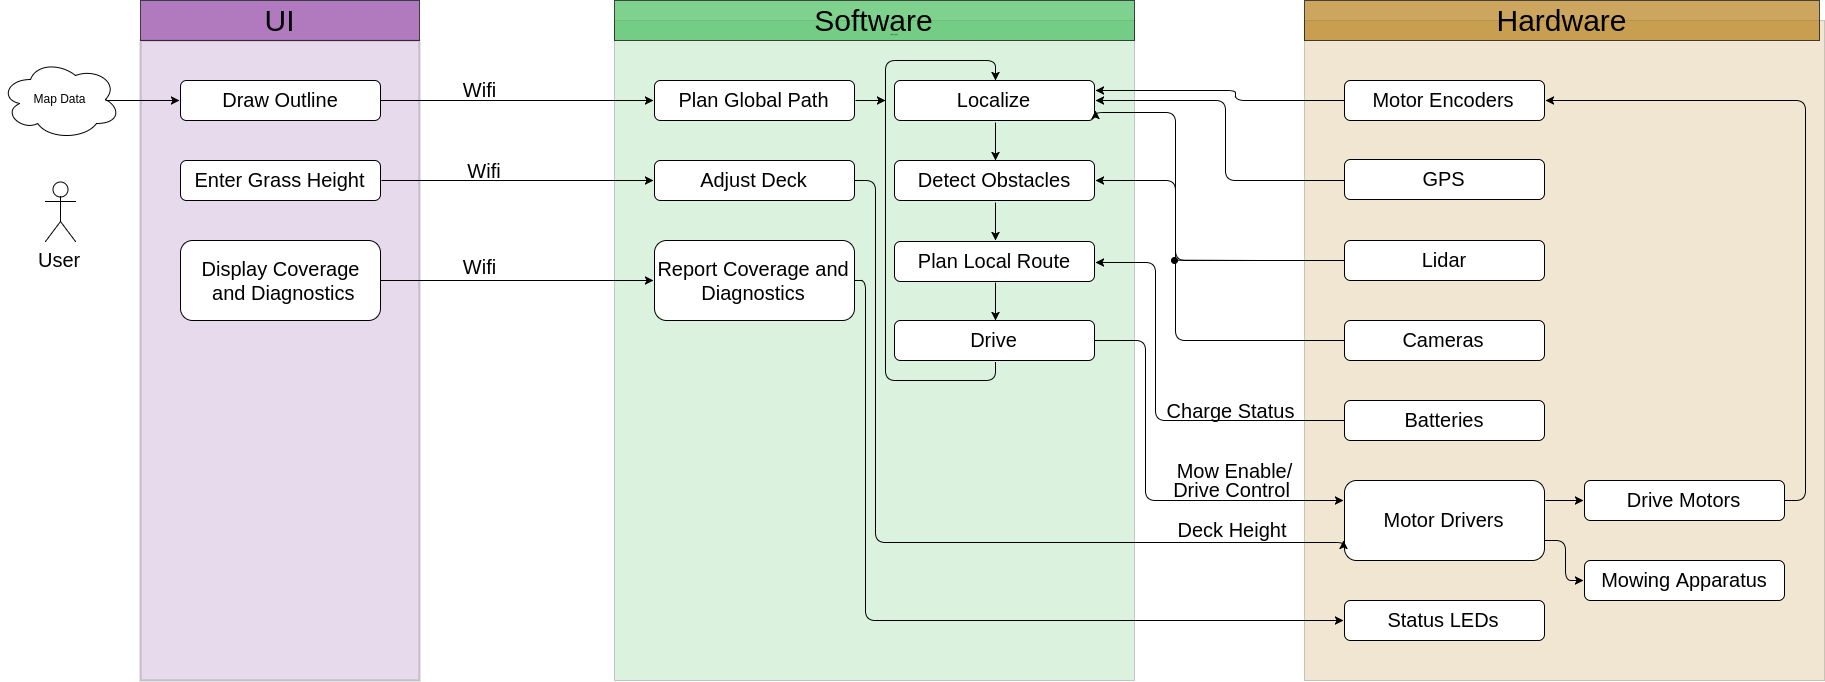
\includegraphics[scale=0.2]{cyberphysical.png}
\caption{Cyberphysical Architecture}
\label{fig:cyberphysical}
\end{figure}

  The user interface and IO subsystems are the contact points for the operator.  The wifi access point allows the user to load mowing boundaries from their laptop or mobile device.  This also enables the user to download coverage reports and diagnostics.  Status LEDs allow the operator to understand the system status at a glance, while safety beacons alert humans to GroundsBot's presence at a distance.\\

  GroundsBot uses its sensor suite to ensure a clean cut. GPS, IMU, and Motor Encoders are used for coarse localization while the cameras are used to ensure optimal grass overlap while cutting.  Cameras and lidar also enable GroundsBot to detect static and dynamic obstacles.\\

  GroundsBot's battery subsystem reports charge status to the CPU to prevent GroundsBot from becoming stranded. The battery subsystem also contains standard protection protocols including charge control, under-voltage lockout, and over-current protection. \\

  The CPU utilizes sensor information for localization, obstacle detection, and planning.  After a local path is devised drive signals are sent to the motors. The CPU also logs coverage data and generates reports.\\

  The Drive Train contains motors and motor drivers to propel GroundsBot across a golf course.  This also encompasses the mowing apparatus and mowing deck height control. \\



\newpage
\section{Subsystem Descriptions}
	\subsection{UI}
	An important aspect of the project is a way for the user to communicate his desired mowing path to the robot. This input method must be separate from the robot itself, allowing the user to be somewhere else as the robot mows autonomously. \\
	
	This will be achieved through a mobile device, either a dedicated tablet or the user's own smartphone. An app or website will be loaded onto this device, and allow for the user to input a map outline that will be communicated to the robot. 
	
	\subsection{Hardware}
		\subsubsection{Platform}
			Based on the trade study, a differential drive system with two drive wheels and one or more caster wheels will be used. Another trade study was used to narrow down the platform to DIY platform instead of a preexisting platform. This custom platform will utilize aluminum extrusions, allowing for easy resizing of the platform as well as easy adjustment of the sensor mounts. Currently, motors and batteries from Discovery Robotics will be integrated, but alternate products may be also be considered. 
			
		\subsubsection{Mower}
			In addition to navigating a plot of grass, the system also needs to mow it. Given that a custom platform will be made, this will be done by attaching an existing electric push mower to the robot platform. Alternatively, it is also possible to attach the blades from a manual reel mower to the platform. 
	
	\subsection{Software}
		\subsubsection{Planner}
			The planner subsystem consists of two parts, a global planner, and  a local planner. The global planner will take the user input from the UI, and translate that into a path that the robot will follow. This involves refining the outline that was provided by the user, and then finding a path that will allow for maximal coverage of the selected area. \\ 
			
			The local planner will be responsible for adapting the route on-the-fly to avoid any obstacles that the robot may encounter. This system will also take care of the driving to and from the dock to the actual cutting area. 
			
		\subsubsection{Localization and Perception}
			An accurate description of the robot's global position and orientation will be obtained from this subsystem. This information may be obtained from a high-accuracy GPS system, such as RTK-GPS, but visual SLAM based methods will also be investigated. \\
			
			The vision system will also be used to detect boundaries of the grass as the robot gets closer to the boundary. For obstacle detection, a trade study determined that a stereo camera system would best fit the detection requirements. However, if needed, a LIDAR may be added to improve the detection accuracy. 
		
		\subsubsection{Mobility}
			The mobility subsystem will be responsible for the control of the robot's motors. Part of this involves the robot going from point A to point B at any given time. Using current position information from localization subsystem, this subsystem will find the next waypoint that will allow for the robot to follow the predetermined plan and then emit the necessary motor control signals to move towards this waypoint. \\
			
			The cutter motor speeds will also be controlled by this subsystem. This subsystem must both detect the speed of the motor, as well as apply the correct motor signals to maintain a constant speed when the cutter encounters an obstacle. 


\newpage
\section{Project Management}
\subsection{Work Plan}
\subsubsection{Tasks}
The GroundsBot work plan is shown in the list below.  The plan is separated into high level categories and underlying subtasks. \\
\begin{outline}[enumerate]
  \1 Chassis
    \2 Complete BOM
    \2 Design Power Distribution and Sensor Integration PCBs % Changed to PCBs from PCBAs because we are "designing PCBs
    \2 Design Chassis
    \2 Design GPS RTK Base Station
    \2 Acquire Parts
    \2 Integrate Subsystems
  \1 Simulation
    \2 Design Simulation Environment
    \2 Complete Cursory Simulations
  \1 Localization
    \2 Integrate GPS + RTK Localization
  \1 Perception
    \2 Develop Static Obstacle Detection
    \2 Develop Dynamic Obstacle Detection
  \1 Planning
    \2 Develop Global Route Planner
    \2 Develop Obstacle Rerouting
  \1 Control
    \2 Develop Motor Control
  \1 UI
    \2 Create Web Application for Mapping
\end{outline}

   
\subsubsection{Schedule}
\noindent
\textbf{Progress Review 1}: The goal for Progress Review 1 is to have all hardware design complete with parts on order. \\
\textbf{Progress Review 2}: The goal for Progress Review 2 is to have an assembled frame/chassis, a full ROS simulation environment, and a completed GPS + RTK base station\\

The full list of milestones is laid out below in Table \ref{Tab:table_milestones}\\ 

\begin{table}[H]
\def\arraystretch{1.2}

\caption{Project Milestones}
\label{Tab:table_milestones}


\begin{tabular}{ll}
\hline
\textbf{Deadline} & \textbf{Milestone}                            \\
\\
Progress Review 1 [OCT 17 2017] & Mechanical CAD Complete \\
    &Electrical CAD Complete                     \\
    &BOM Complete                                \\
    &Parts Ordered                               \\
    &ROS Environment Initialized                 \\
                                               \\
Progress Review 2 [OCT 26 2017] & Chassis Assembled with Mowing Apparatus     \\
    &ROS Simulation Environment Complete         \\
    &GPS RTK Base Station Complete               \\
                                              \\ 
Progress Review 3 [NOV 7 2017] 
    &GroundsBot System Integration Complete      \\
    &GPS RTK Integration Complete                \\
    &Control Systems Demo Complete               \\
                                              \\
Progress Review 4 [NOV 21 2017] 
  
    &GroundsBot Accepts GPS Waypoints            \\
    &GroundsBot Follows GPS waypoints            \\
    &Teleoperation Test Complete                 \\
                                               \\
Fall Validation Experiment [NOV 28 2017] 
 
    &GroundsBot Follows Route From Web App       \\
    &GroundsBot Differentiates Grass From Other Objects \\
                                            \\
                                            
January 2018 Milestone 

    &Global Planning Algorithm Complete          \\
    &Static and Dynamic Obstacle Detection Complete\\
                                               \\
February 2018 Milestone 
  
    &Read User Map Input                        \\
    &GroundsBot Reroutes Around Obstacles       \\
                                              \\
March 2018 
  
    &Full Mapping UI Complete                   \\
    &GroundsBot Autonomously Cuts Lot           \\
                                              \\
April 2018 

    &Final System Tests Complete                \\                                            \\
\end{tabular}

\end{table}

\subsubsection{Progress Reviews}

\subsection{System Validation Experiments}
\subsubsection{Fall Validation Experiment}

	The aim of the fall validation experiment is to test individual subsystems. As such many of the systems requirements set for GroundsBot will not be fully met. All tests to be performed have been designed to indicate significant progress towards reaching the system requirements. More specifically the team plans to test the base functionality of the mobility, localization, planning, and perception subsystems of GroundsBot. The details of the test are laid out below.
\\
\begin{center}
\textbf{Test 1:}
\end{center}
\textbf{Location:} Field by Doherty Apartments
\\
\textbf{Equipment:} GroundsBot, GroundsBot dock/RTK base station, laptop
\begin{enumerate}
  \item Power on GroundsBot next to its docking station
  \item Establish connection between GroundsBot and mobile device
  \item Input GPS waypoints following a typical zigzag pattern a groundskeeper might make when mowing a lawn
  \item Send waypoints to GroundsBot
  \item GroundsBot will navigate to each waypoint entered, in the order they were entered
  \item Once the last waypoint is reached, GroundsBot will navigate back to the docking station (Note: the docking station will not be one of the entered waypoints)
\end{enumerate}

\begin{center}
\textbf{Test 2:}
\end{center}
Test 2 has been designed to demonstrate base functionality of the perception subsystem. The team will present perception algorithm capable of differentiating between grass(i.e. a mowable surface) and non-grass (i.e. a non-mowable surface.) This test will be performed outside of the fall validation experiment and a replay of the test will be displayed during the fall validation experiment.

\subsubsection{Spring Validation Experiment}

	The spring validation experiment will be when the team will test the full GroundsBot system to demonstrate that all system requirements have been met. The details of the test are laid out below.
\begin{center}
\textbf{Test 1: }
\end{center}
\textbf{Location:} Field by Doherty Apartments
\textbf{Equipment:} GroundsBot, GroundsBot dock/RTK base station, mobile device
\begin{enumerate}
  \item Power on GroundsBot next to its docking station
  \item Open UI on mobile interface and establish a connection with GroundsBot
  \item Have a new user (someone not on Team A) use the UI to draw an outline of the area to be mowed on a map
  \begin{enumerate}
    \item Area should include both static obstacles and a non-mowable surface (i.e. concrete)
  \end{enumerate}
  \item Use the UI to submit the mowing area to GroundsBot
  \item GroundsBot will develop a coverage plan of the area input by the user
  \item GroundsBot will navigate to the area to be mowed
  \item Once it has reached the edge of the mowing area it will begin mowing
  \item GroundsBot will detect and avoid any obstacles it comes across while mowing and will also only mow where there is grass
  \item Once GroundsBot has mowed the whole area it will return to the docking station
  \item GroundsBot will generate and transmit a coverage report to the UI indicating areas it could not mow
\end{enumerate}
\subsection{Team Member Responsibilities}
\subsection{Provisional BOM}
\begin{table}[H]
\centering
\def\arraystretch{1.1}
\caption{Provisional BOM}
\label{Tab:provisional_bom}
\begin{tabular}{ llccl }
\hline
    \textbf{Manufacturer} & \textbf{Part No.} & \textbf{QTY} & \textbf{Cost} & \textbf{Description}\\
    \\[-.8ex]
    SuperDroid Robots & TD-111-135 & 1 & \$900 & Wheelchair Motors \& Encoders \\
	SuperDroid Robots & TE-240-030 & 1 & \$330 & Motor Controller \\
	SuperDroid Robots & TD-178-000 & 1 & \$150 & 13" Tiller Tires and Mounting \\
	Caster Connection & S-5210-PRB & 1 & \$70 & 10" Pneumatic Swivel Caster \\
	Smart Battery & SB2425 & 1 & \$700 & 24V 25aH Battery \\
    Smart Battery & DP-RS2 & 1 & \$165 & Battery Charger \\
    NVIDIA & Jetson TX2 Dev Kit & 1 & \$560 &  Embedded GPU \\
	ITEM & Extrusion & 1 & \$400 & Extrusions and Joints \\
	McMaster-Carr & Mechanical Components & 1 & \$500 & Misc Fasteners, Bearings \\
	DigiKey & Electrical Components & 1 & \$600 & Misc Connectors, Components \\[.5ex]
	\hline 
	\\[-2ex]
	Total: &&& \$4,375 &\\
	
    
\end{tabular}
\end{table}

\subsection{Risk Management}
\begin{table}[H]
\def\arraystretch{1.7}

\begin{tabular}{p{7cm}p{6cm}c}
\textbf{Risk} & \textbf{Management Strategy} & \textbf{Risk Category}\\
\hline 
\textbf{Too Few Features for Perception:} 
If we cannot consistently detect grass from non-grass features, perception subsystem will not be able to direct platform accurately
&
Install infrastructure such as fiducials to assist system in recognizing objects.
&
Technical\\

\textbf{Team Falling Behind Due to Work:} 
Team may overestimate capability and overwhelm itself with assignments.
&
Prepare for risk by managing tasks and using buffer weeks.  Mitigate effect by delaying milestones or cutting compromising targets.
&
Schedule\\
\textbf{Localization Poor for Following Edges:} 
If our localization algorithms cannot accurately follow edge of lawn, system will not mow lawn effectively.
&
Prepare by understanding criticality of localization.  Mitigate effect by changing scope of mowing problem or adding infrastructure to assist.
&
Technical\\
\textbf{Injury from Spinning Blade:} 

Our system has a dangerous cutting instrument.  It can injure a team member or a bystander.
&
Prepare by making sure team understands the risk of spinning blade.  Put warning lights and sounds to alert bystanders when testing.
&
Technical\\

\textbf{Poor Weather for Validation Experiments:} 
Poor weather on demonstration days would prevent us from system from performing.
&1
Team monitors upcoming weather before validation experiments.  Communicates with instructing team to reschedule if concerned by inclement weather.
&
Schedule\\

\textbf{Team Member Has Family Constraints:} 
Any team member could experience a family emergency or reponsibility that occupies their time and focus.  One specific concern is Josh's wife is pregnant and expecting in December.
&
Mitigate the effect on entire team by spreading work across several team members and communicating consistently with absent team member to keep them in the loop.
&
Personal\\

\textbf{Platform Devastating Event:} 
Platform could have electrical, thermal, or kinetic event that leads to its destruction.
&
Team designs platform with risk in mind, and manages parts reserve to quickly rebuild platform if necessary.
&
Technical\\

\textbf{Subsystem Harder Than Expected:} 
Any subsystem could require more work than expected, taking away focus from other subsystems.
&
Team can prepare by focusing on critical subsystems first, and may revise scope related to subsystem if necessary.
&
Technical\\

\textbf{Not Enough Capital for Development:} 
There is a risk our system requires more money than initially allocated.
&
To mitigate the effect of this event, team will maintain strong relationship with sponsor by providing consistent communication of development progress. Team may also reach out to other sponsors or donors.
&
Schedule\\
\end{tabular}
\end{table}

\begingroup
\newpage
\section{References}
\renewcommand{\section}[2]{}% %Suppress bibliography header, doesn't work with toc
\begin{thebibliography}{}
\bibitem{clubbenchmarking} 
http://www.clubbenchmarking.com/blog/golf-course-maintenance-how-much-should-you-spend
\bibitem{husky} 
https://www.clearpathrobotics.com/husky-unmanned-ground-vehicle-robot/
\bibitem{husqvarna} 
http://www.husqvarna.com/us/products/robotic-lawn-mowers/
\bibitem{swiftnav} 
https://www.swiftnav.com/store?category=GNSS+Modules
\bibitem{superdroid} 
https://www.superdroidrobots.com/shop/item.aspx/prebuilt-2wd-66in-lawn-mower-wc-sold/1983/
\bibitem{interview-duxbury} 
Duxbury, Jeff [Bob O’Connor Golf Course Superintendent]. (2017, September 16). Personal interview.
\bibitem{interview-guenther} 
Guenther, Steve [Carnegie Mellon University Director of Facilities Operations]. (2017, September 22). Personal interview.
\bibitem{interview-zang} 
Zang, Jason [Allegheny County Maintenance Manager]. (2017, September 25). Phone interview.
\end{thebibliography}
\endgroup

\end{document}
